\documentclass[11pt]{article}
\usepackage[textwidth=18.0cm, textheight=23.0cm, top=2.0cm]{geometry}
\usepackage{pst-all}
\usepackage{amssymb}
\usepackage{tikz}
\usepackage{underscore}\begin{document}
\pagestyle{empty}


ClassName: \underline{\textbf{Class_03.2bp-16}}
\par
BinSize: \underline{\textbf{40 × 40}}
\par
ReduceSize: \underline{\textbf{40 × 40}}
\par
TypeNum: \underline{\textbf{39}}
\par
Num: \underline{\textbf{40}}
\par
OutS: \underline{\textbf{12800}}
\par
InS: \underline{\textbf{11621}}
\par
Rate: \underline{\textbf{0.908}}
\par
UB: \underline{\textbf{8}}
\par
LB0: \underline{\textbf{8}}
\par
LB: \underline{\textbf{8}}
\par
LBWithCut: \underline{\textbf{8}}
\par
NodeCut: \underline{\textbf{0}}
\par
ExtendedNodeCnt: \underline{\textbf{1}}
\par
GenNodeCnt: \underline{\textbf{1}}
\par
PrimalNode: \underline{\textbf{0}}
\par
ColumnCount: \underline{\textbf{8}}
\par
TotalCutCount: \underline{\textbf{0}}
\par
RootCutCount: \underline{\textbf{0}}
\par
LPSolverCnt: \underline{\textbf{1}}
\par
PricingSolverCnt: \underline{\textbf{0}}
\par
BranchAndBoundNum: \underline{\textbf{1}}
\par
isOpt: \underline{\textbf{true}}
\par
TimeOnInitSolution: \underline{\textbf{600.000 s}}
\par
TimeOnPrimal: \underline{\textbf{0.000 s}}
\par
TimeOnPricing: \underline{\textbf{0.000 s}}
\par
TimeOnRmp: \underline{\textbf{0.062 s}}
\par
TotalTime: \underline{\textbf{600.391 s}}
\par
\newpage


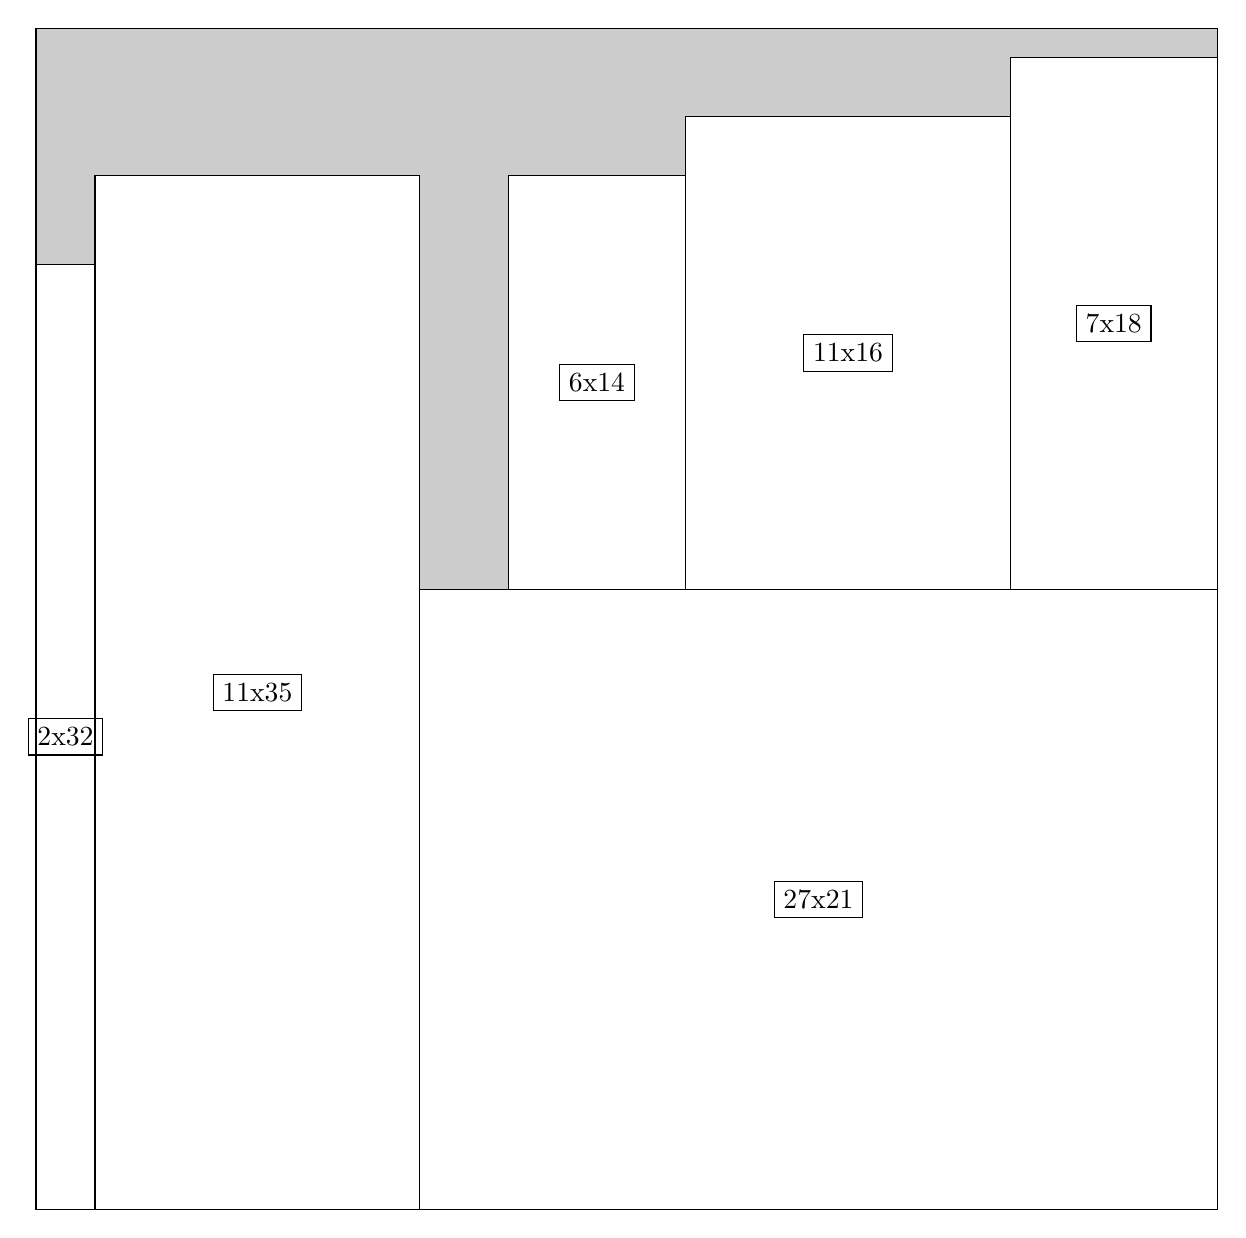
\begin{tikzpicture}[shorten >=1pt,scale=1.0,every node/.style={scale=1.0},->]
\tikzstyle{vertex}=[circle,fill=black!25,minimum size=14pt,inner sep=0pt]
\filldraw[fill=gray!40!white, draw=black] (0,0) rectangle (15.0,15.0);
\foreach \name/\x/\y/\w/\h in {27x21/4.875/0.0/10.125/7.875,7x18/12.375/7.875/2.625/6.75,11x16/8.25/7.875/4.125/6.0,6x14/6.0/7.875/2.25/5.25,11x35/0.75/0.0/4.125/13.125,2x32/0.0/0.0/0.75/12.0}
\filldraw[fill=white!40!white, draw=black] (\x,\y) rectangle node[draw] (\name) {\name} ++(\w,\h);
\end{tikzpicture}


w =27 , h =21 , x =13 , y =0 , v =567
\par
w =7 , h =18 , x =33 , y =21 , v =126
\par
w =11 , h =16 , x =22 , y =21 , v =176
\par
w =6 , h =14 , x =16 , y =21 , v =84
\par
w =11 , h =35 , x =2 , y =0 , v =385
\par
w =2 , h =32 , x =0 , y =0 , v =64
\par
\newpage


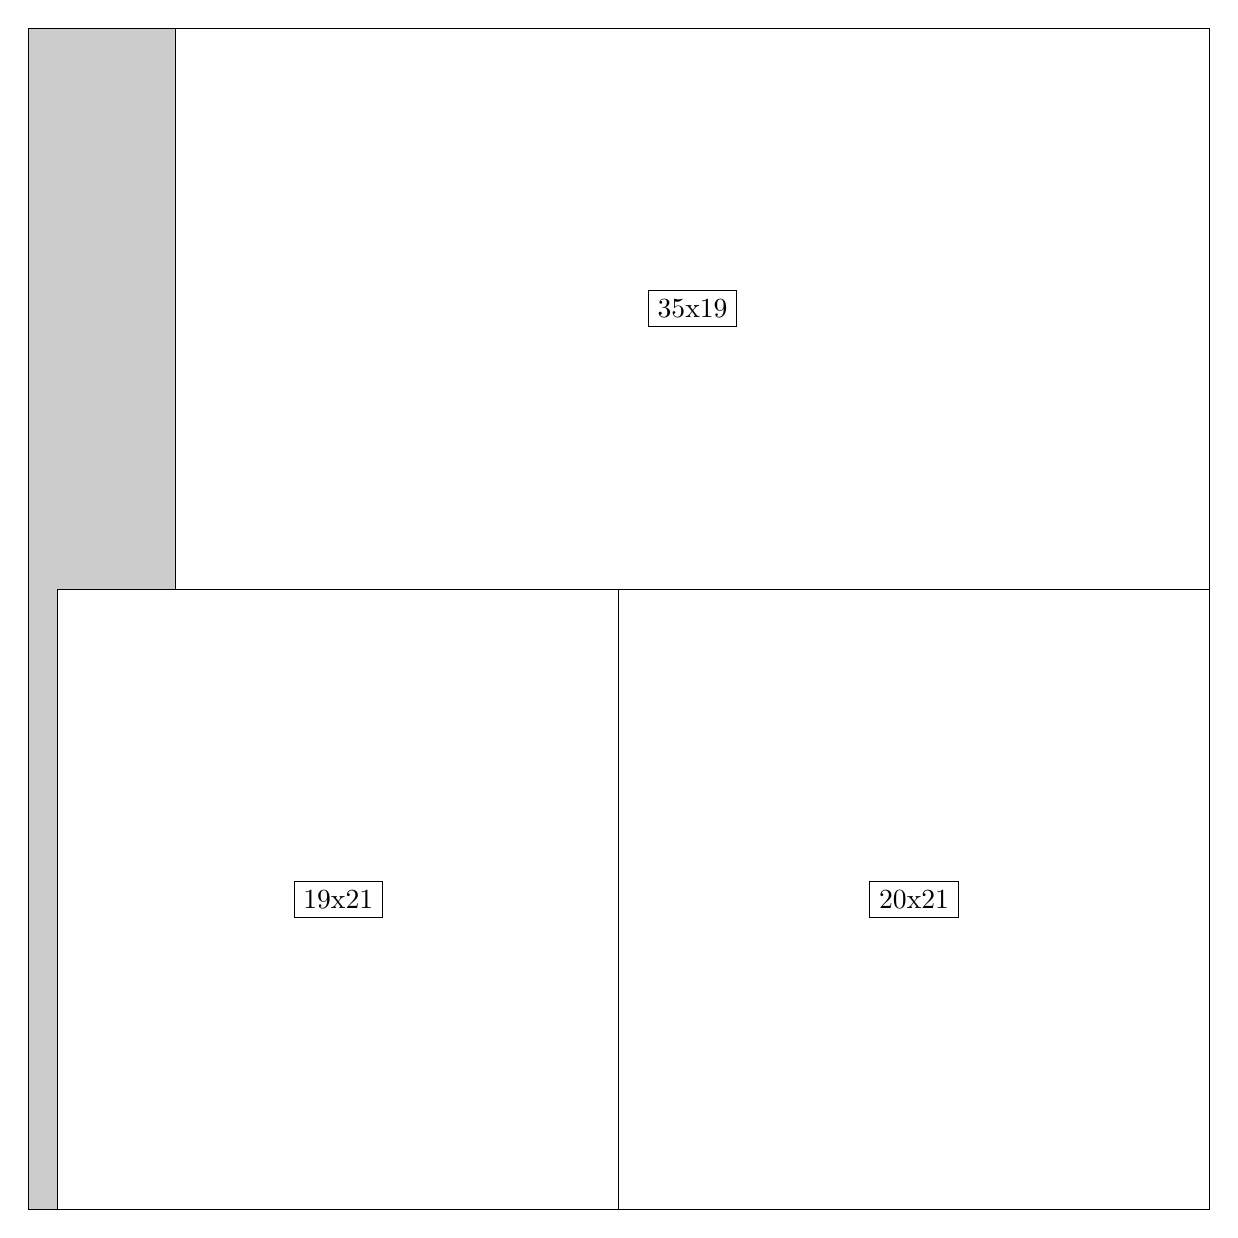
\begin{tikzpicture}[shorten >=1pt,scale=1.0,every node/.style={scale=1.0},->]
\tikzstyle{vertex}=[circle,fill=black!25,minimum size=14pt,inner sep=0pt]
\filldraw[fill=gray!40!white, draw=black] (0,0) rectangle (15.0,15.0);
\foreach \name/\x/\y/\w/\h in {20x21/7.5/0.0/7.5/7.875,19x21/0.375/0.0/7.125/7.875,35x19/1.875/7.875/13.125/7.125}
\filldraw[fill=white!40!white, draw=black] (\x,\y) rectangle node[draw] (\name) {\name} ++(\w,\h);
\end{tikzpicture}


w =20 , h =21 , x =20 , y =0 , v =420
\par
w =19 , h =21 , x =1 , y =0 , v =399
\par
w =35 , h =19 , x =5 , y =21 , v =665
\par
\newpage


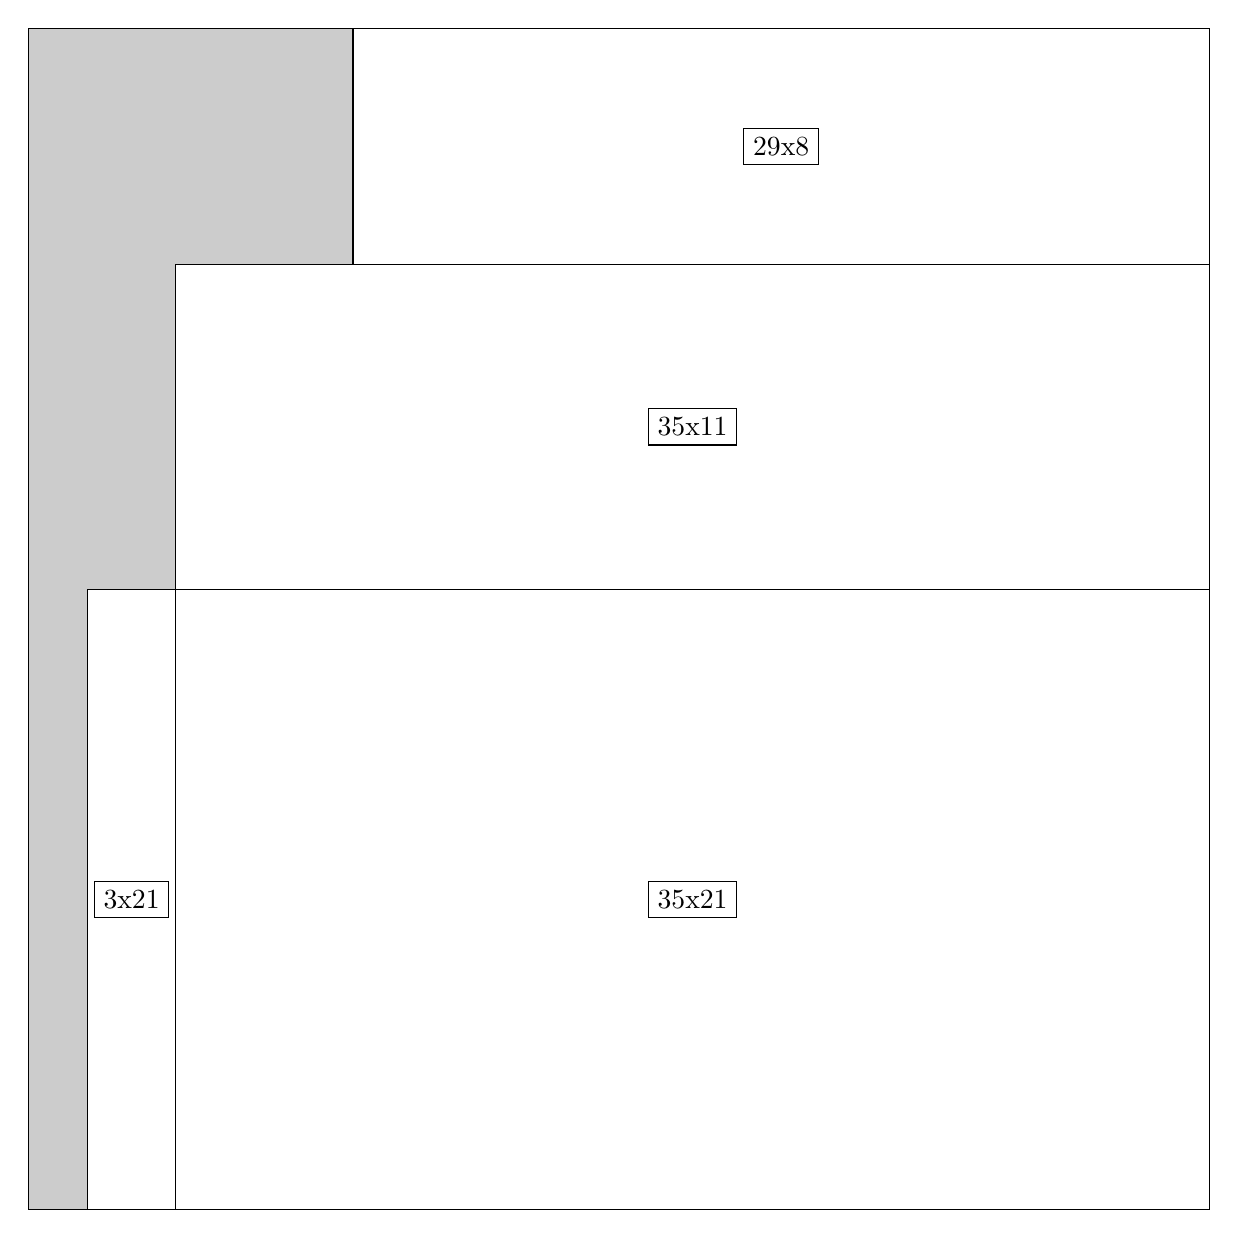
\begin{tikzpicture}[shorten >=1pt,scale=1.0,every node/.style={scale=1.0},->]
\tikzstyle{vertex}=[circle,fill=black!25,minimum size=14pt,inner sep=0pt]
\filldraw[fill=gray!40!white, draw=black] (0,0) rectangle (15.0,15.0);
\foreach \name/\x/\y/\w/\h in {35x21/1.875/0.0/13.125/7.875,3x21/0.75/0.0/1.125/7.875,35x11/1.875/7.875/13.125/4.125,29x8/4.125/12.0/10.875/3.0}
\filldraw[fill=white!40!white, draw=black] (\x,\y) rectangle node[draw] (\name) {\name} ++(\w,\h);
\end{tikzpicture}


w =35 , h =21 , x =5 , y =0 , v =735
\par
w =3 , h =21 , x =2 , y =0 , v =63
\par
w =35 , h =11 , x =5 , y =21 , v =385
\par
w =29 , h =8 , x =11 , y =32 , v =232
\par
\newpage


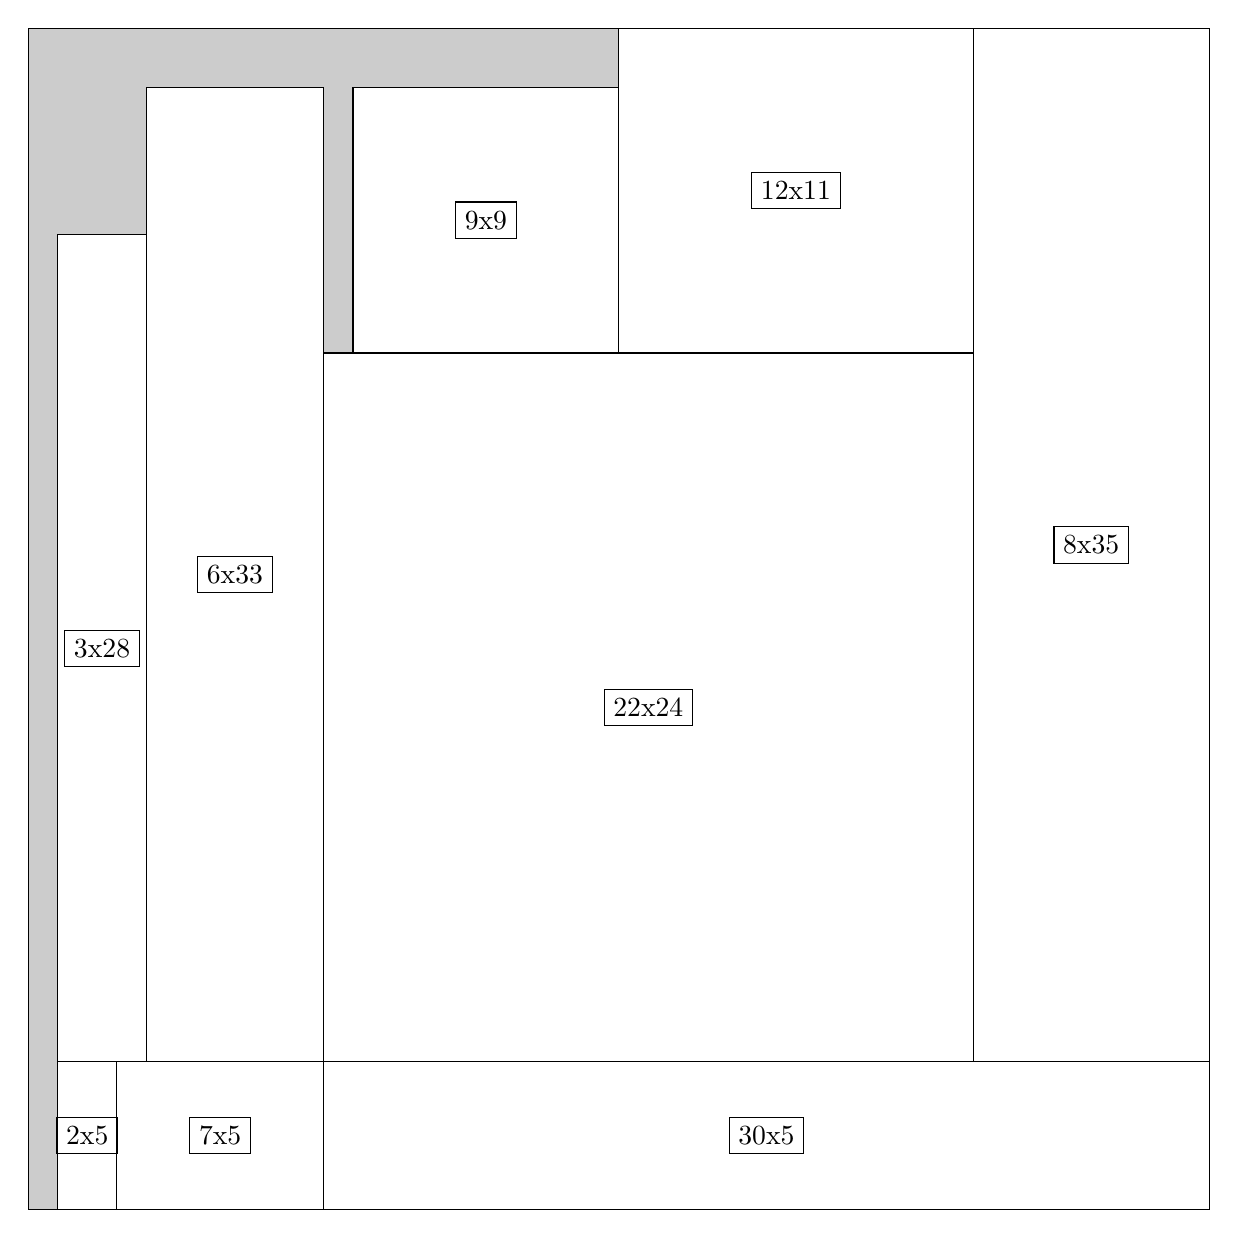
\begin{tikzpicture}[shorten >=1pt,scale=1.0,every node/.style={scale=1.0},->]
\tikzstyle{vertex}=[circle,fill=black!25,minimum size=14pt,inner sep=0pt]
\filldraw[fill=gray!40!white, draw=black] (0,0) rectangle (15.0,15.0);
\foreach \name/\x/\y/\w/\h in {30x5/3.75/0.0/11.25/1.875,7x5/1.125/0.0/2.625/1.875,2x5/0.375/0.0/0.75/1.875,8x35/12.0/1.875/3.0/13.125,22x24/3.75/1.875/8.25/9.0,12x11/7.5/10.875/4.5/4.125,9x9/4.125/10.875/3.375/3.375,6x33/1.5/1.875/2.25/12.375,3x28/0.375/1.875/1.125/10.5}
\filldraw[fill=white!40!white, draw=black] (\x,\y) rectangle node[draw] (\name) {\name} ++(\w,\h);
\end{tikzpicture}


w =30 , h =5 , x =10 , y =0 , v =150
\par
w =7 , h =5 , x =3 , y =0 , v =35
\par
w =2 , h =5 , x =1 , y =0 , v =10
\par
w =8 , h =35 , x =32 , y =5 , v =280
\par
w =22 , h =24 , x =10 , y =5 , v =528
\par
w =12 , h =11 , x =20 , y =29 , v =132
\par
w =9 , h =9 , x =11 , y =29 , v =81
\par
w =6 , h =33 , x =4 , y =5 , v =198
\par
w =3 , h =28 , x =1 , y =5 , v =84
\par
\newpage


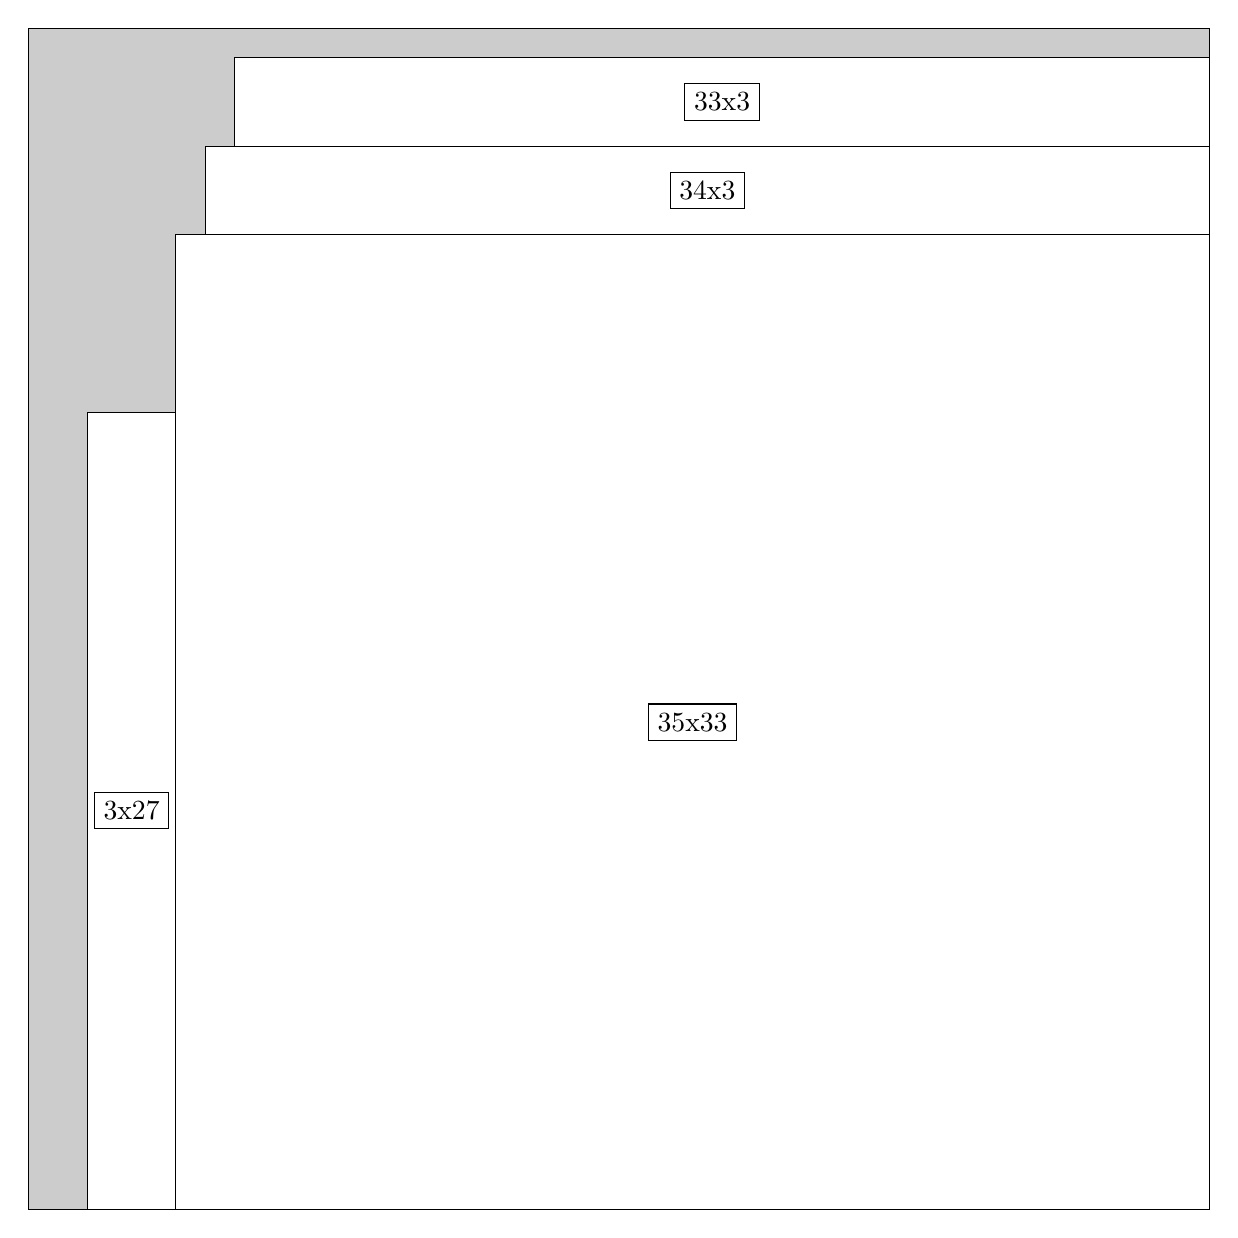
\begin{tikzpicture}[shorten >=1pt,scale=1.0,every node/.style={scale=1.0},->]
\tikzstyle{vertex}=[circle,fill=black!25,minimum size=14pt,inner sep=0pt]
\filldraw[fill=gray!40!white, draw=black] (0,0) rectangle (15.0,15.0);
\foreach \name/\x/\y/\w/\h in {35x33/1.875/0.0/13.125/12.375,3x27/0.75/0.0/1.125/10.125,34x3/2.25/12.375/12.75/1.125,33x3/2.625/13.5/12.375/1.125}
\filldraw[fill=white!40!white, draw=black] (\x,\y) rectangle node[draw] (\name) {\name} ++(\w,\h);
\end{tikzpicture}


w =35 , h =33 , x =5 , y =0 , v =1155
\par
w =3 , h =27 , x =2 , y =0 , v =81
\par
w =34 , h =3 , x =6 , y =33 , v =102
\par
w =33 , h =3 , x =7 , y =36 , v =99
\par
\newpage


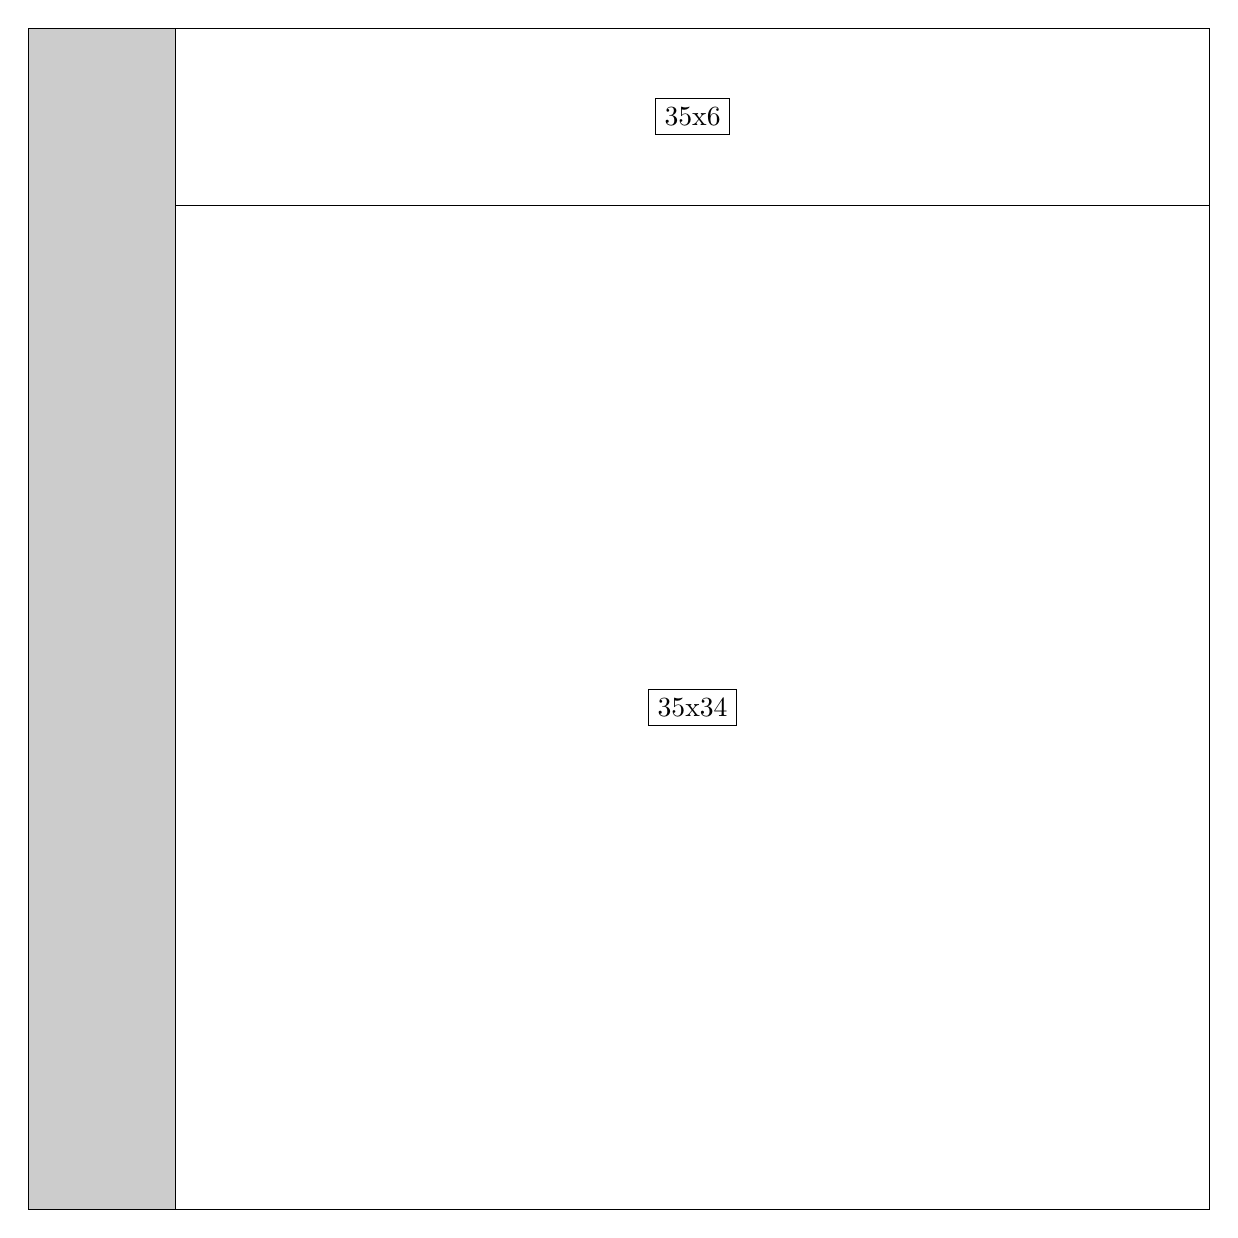
\begin{tikzpicture}[shorten >=1pt,scale=1.0,every node/.style={scale=1.0},->]
\tikzstyle{vertex}=[circle,fill=black!25,minimum size=14pt,inner sep=0pt]
\filldraw[fill=gray!40!white, draw=black] (0,0) rectangle (15.0,15.0);
\foreach \name/\x/\y/\w/\h in {35x34/1.875/0.0/13.125/12.75,35x6/1.875/12.75/13.125/2.25}
\filldraw[fill=white!40!white, draw=black] (\x,\y) rectangle node[draw] (\name) {\name} ++(\w,\h);
\end{tikzpicture}


w =35 , h =34 , x =5 , y =0 , v =1190
\par
w =35 , h =6 , x =5 , y =34 , v =210
\par
\newpage


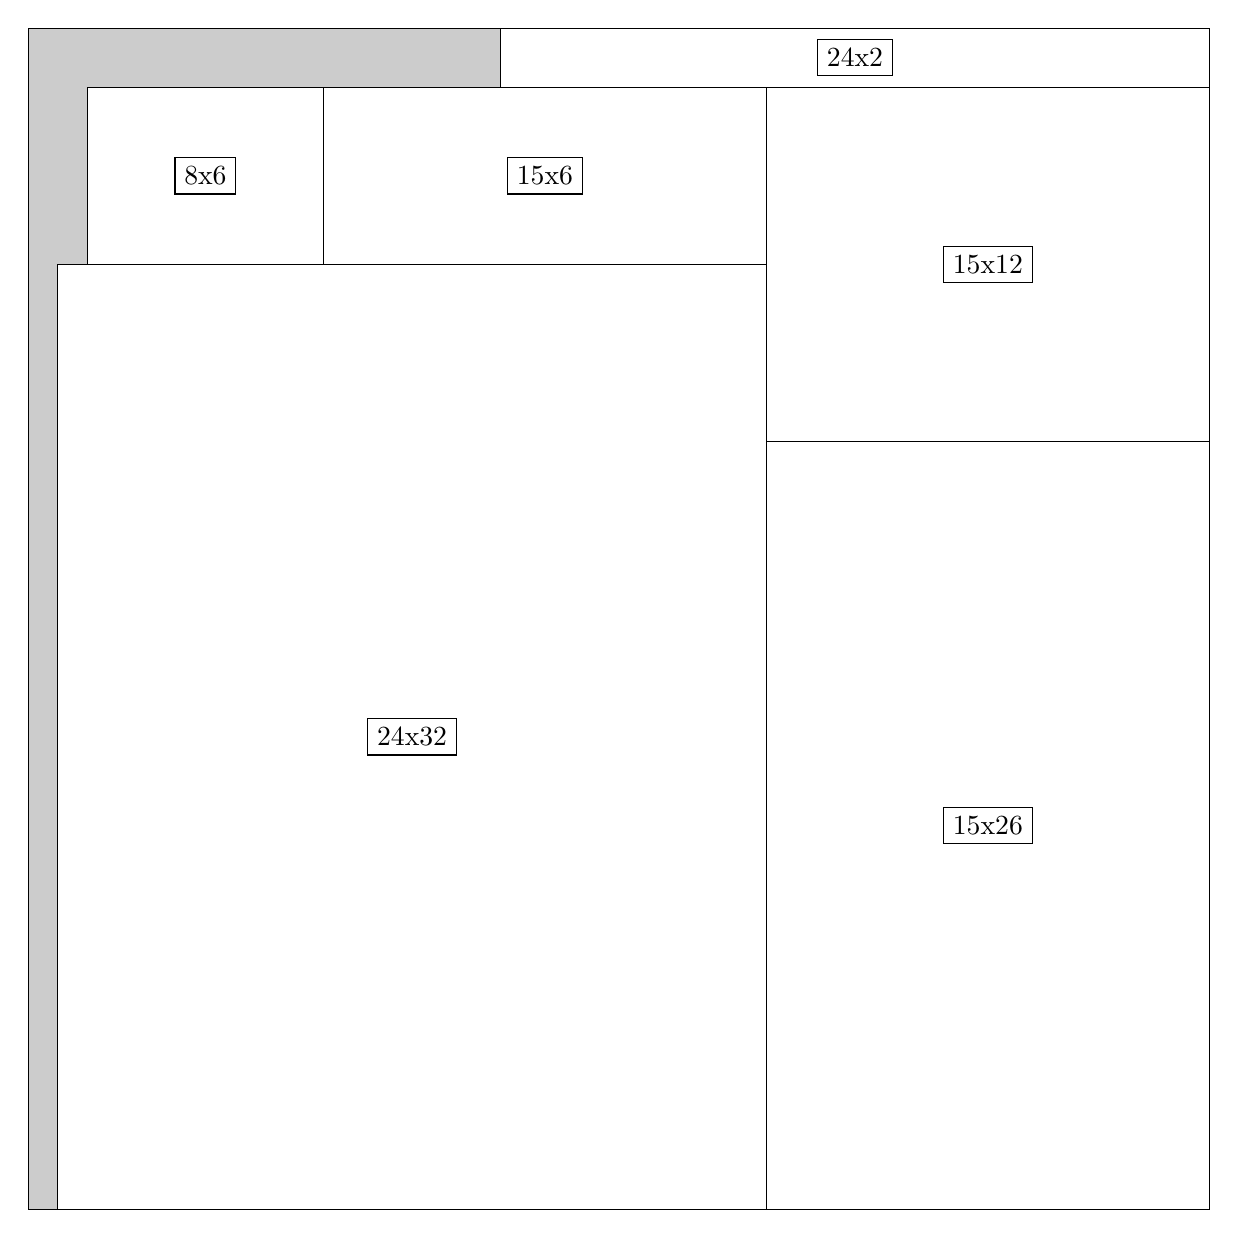
\begin{tikzpicture}[shorten >=1pt,scale=1.0,every node/.style={scale=1.0},->]
\tikzstyle{vertex}=[circle,fill=black!25,minimum size=14pt,inner sep=0pt]
\filldraw[fill=gray!40!white, draw=black] (0,0) rectangle (15.0,15.0);
\foreach \name/\x/\y/\w/\h in {15x26/9.375/0.0/5.625/9.75,15x12/9.375/9.75/5.625/4.5,24x32/0.375/0.0/9.0/12.0,15x6/3.75/12.0/5.625/2.25,8x6/0.75/12.0/3.0/2.25,24x2/6.0/14.25/9.0/0.75}
\filldraw[fill=white!40!white, draw=black] (\x,\y) rectangle node[draw] (\name) {\name} ++(\w,\h);
\end{tikzpicture}


w =15 , h =26 , x =25 , y =0 , v =390
\par
w =15 , h =12 , x =25 , y =26 , v =180
\par
w =24 , h =32 , x =1 , y =0 , v =768
\par
w =15 , h =6 , x =10 , y =32 , v =90
\par
w =8 , h =6 , x =2 , y =32 , v =48
\par
w =24 , h =2 , x =16 , y =38 , v =48
\par
\newpage


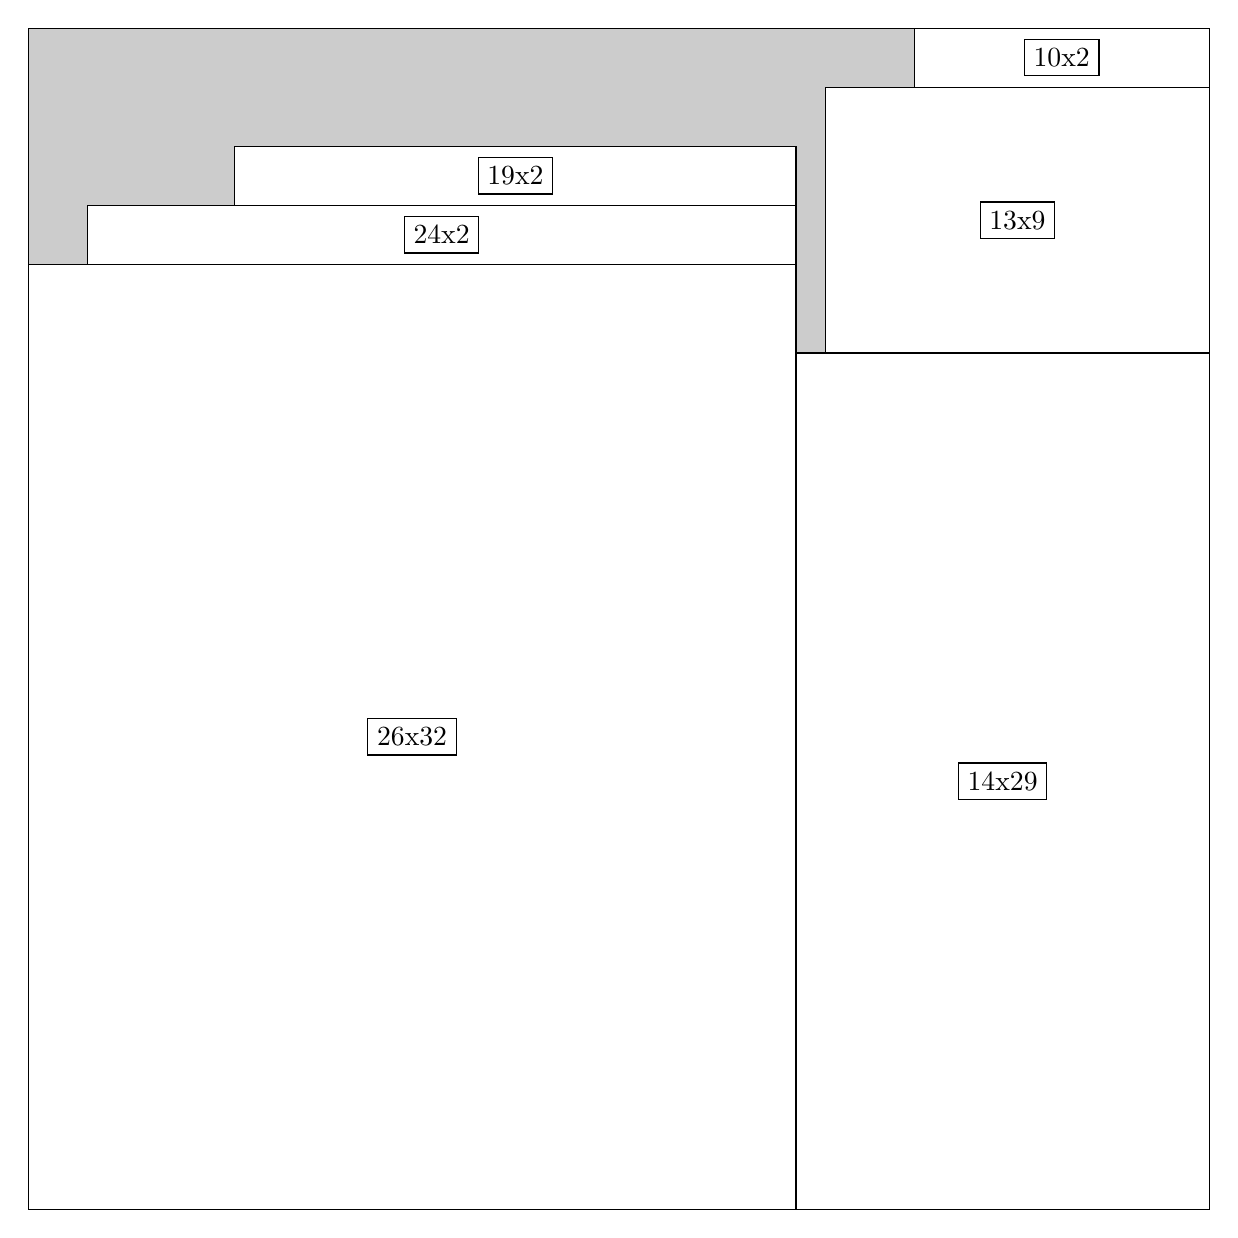
\begin{tikzpicture}[shorten >=1pt,scale=1.0,every node/.style={scale=1.0},->]
\tikzstyle{vertex}=[circle,fill=black!25,minimum size=14pt,inner sep=0pt]
\filldraw[fill=gray!40!white, draw=black] (0,0) rectangle (15.0,15.0);
\foreach \name/\x/\y/\w/\h in {14x29/9.75/0.0/5.25/10.875,13x9/10.125/10.875/4.875/3.375,10x2/11.25/14.25/3.75/0.75,26x32/0.0/0.0/9.75/12.0,24x2/0.75/12.0/9.0/0.75,19x2/2.625/12.75/7.125/0.75}
\filldraw[fill=white!40!white, draw=black] (\x,\y) rectangle node[draw] (\name) {\name} ++(\w,\h);
\end{tikzpicture}


w =14 , h =29 , x =26 , y =0 , v =406
\par
w =13 , h =9 , x =27 , y =29 , v =117
\par
w =10 , h =2 , x =30 , y =38 , v =20
\par
w =26 , h =32 , x =0 , y =0 , v =832
\par
w =24 , h =2 , x =2 , y =32 , v =48
\par
w =19 , h =2 , x =7 , y =34 , v =38
\par
\newpage


\end{document}